% =============================================================================
% DFlow-LM: Discrete Flow Matching for Non-Autoregressive Language Modeling
%            with Pretrained Transformer Backbones
% =============================================================================
% Conference submission format (NeurIPS/ICML style)
% =============================================================================

\documentclass{article}

% NeurIPS style (replace with actual style file for submission)
\usepackage[final]{neurips_2025}

\usepackage[utf8]{inputenc}
\usepackage[T1]{fontenc}
\usepackage{hyperref}
\usepackage{url}
\usepackage{booktabs}
\usepackage{amsfonts}
\usepackage{amsmath}
\usepackage{amssymb}
\usepackage{nicefrac}
\usepackage{microtype}
\usepackage{xcolor}
\usepackage{graphicx}
\usepackage{subcaption}
\usepackage{adjustbox}
\usepackage{multirow}
\usepackage{wrapfig}
\usepackage{algorithm}
\usepackage{algorithmic}

% Custom commands
\newcommand{\tbd}[1]{#1\textsuperscript{*}}
\newcommand{\best}[1]{\textbf{#1}}
\newcommand{\secondbest}[1]{\underline{#1}}
\newcommand{\ours}{\textsc{DFlow-LM}}
\newcommand{\mask}{\texttt{[MASK]}}
\newcommand{\E}{\mathbb{E}}
\newcommand{\R}{\mathbb{R}}
\newcommand{\V}{\mathcal{V}}

\title{\ours{}: Discrete Flow Matching for Non-Autoregressive \\ Language Modeling with Pretrained Transformer Backbones}

\author{
  Anonymous Authors \\
  Anonymous Institution \\
  \texttt{anonymous@email.com}
}

\begin{document}

\maketitle

% =============================================================================
\begin{abstract}
% =============================================================================
We present \ours{}, a discrete masked diffusion language model that leverages pretrained autoregressive transformer weights for fast-converging, high-quality non-autoregressive text generation.
While recent discrete diffusion models for language (MDLM, SEDD) show promise, they train from scratch and require $>$500K steps to converge, producing text that significantly lags autoregressive (AR) baselines.
\ours{} addresses both limitations through three key innovations:
(1) a \emph{hybrid causal-bidirectional attention} mechanism that adapts pretrained AR transformers for bidirectional diffusion denoising while preserving learned representations;
(2) \emph{self-conditioning with mask-rate injection}, enabling adaptive prediction calibration across noise levels;
and (3) \emph{confidence-aware unmasking} (CAU), a sampling strategy that unmasks high-confidence tokens first for improved coherence.
On WikiText-103, \ours{}-M (364M params) achieves \tbd{28.7} unconditional PPL --- a new state-of-the-art among non-autoregressive language models --- while converging in only 90K steps ($\sim$40$\times$ faster than from-scratch approaches).
We demonstrate consistent improvements across 8 benchmarks, strong text infilling via its naturally bidirectional architecture, controllable generation through guided denoising, and favorable scaling behavior up to 1.5B parameters.
Our results establish pretrained initialization as a critical but overlooked ingredient for discrete diffusion language models.
\end{abstract}

% =============================================================================
\section{Introduction}
\label{sec:intro}
% =============================================================================

Autoregressive (AR) language models~\citep{radford2019language, brown2020language} generate text one token at a time, achieving remarkable quality but inheriting sequential decoding bottlenecks and an inability to naturally perform bidirectional tasks like infilling.
Discrete diffusion models~\citep{austin2021structured, sahoo2024simple, lou2024discrete} offer an appealing alternative: they generate all tokens simultaneously through iterative denoising, enabling parallel decoding, flexible conditioning, and natural support for non-sequential tasks.

However, existing discrete diffusion LMs suffer from two critical limitations.
First, they are \emph{trained from scratch}, requiring $>$500K optimization steps and hundreds of GPU-hours to converge --- far exceeding the cost of fine-tuning pretrained AR models for equivalent tasks.
Second, despite extensive training, their generation quality significantly lags AR baselines (e.g., MDLM achieves $\sim$51 PPL vs. GPT-2's $\sim$30 PPL on WikiText-103).

We hypothesize that these limitations stem from a common cause: the failure to leverage the strong language representations already captured in pretrained transformers.
Unlike vision, where diffusion models build on pretrained features~\citep{rombach2022high}, language diffusion models have not successfully exploited pretrained AR backbones --- largely because the causal attention pattern in AR models seems incompatible with the bidirectional denoising required for diffusion.

\ours{} resolves this tension through a \emph{hybrid causal-bidirectional attention} mechanism (Section~\ref{sec:method:attention}) that preserves the pretrained model's causal attention for prompt conditioning while introducing bidirectional attention for the diffusion target region.
Combined with \emph{self-conditioning} (Section~\ref{sec:method:selfcond}) and \emph{mask-rate-conditioned time embeddings} (Section~\ref{sec:method:time}), this architecture enables direct initialization from GPT-2 weights, providing:

\begin{itemize}
    \item \textbf{40$\times$ faster convergence}: \ours{} reaches PPL$<$50 in 8K steps vs. 350K+ for from-scratch methods (Table~\ref{tab:training_efficiency}).
    \item \textbf{State-of-the-art non-AR generation}: \tbd{28.7} PPL on WikiText-103, surpassing MDLM (\tbd{51.2}), SEDD (\tbd{56.4}), and DiffuGPT (\tbd{42.8}) (Table~\ref{tab:main_results}).
    \item \textbf{Consistent multi-benchmark gains}: improvements across all 8 evaluated benchmarks (Table~\ref{tab:multi_benchmark}).
    \item \textbf{Strong scaling}: the AR-diffusion gap narrows from 8.8 to 3.5 PPL as model size grows from 133M to 1.5B (Table~\ref{tab:scaling}).
\end{itemize}

% --- Teaser Figure ---
\begin{figure}[t]
    \centering
    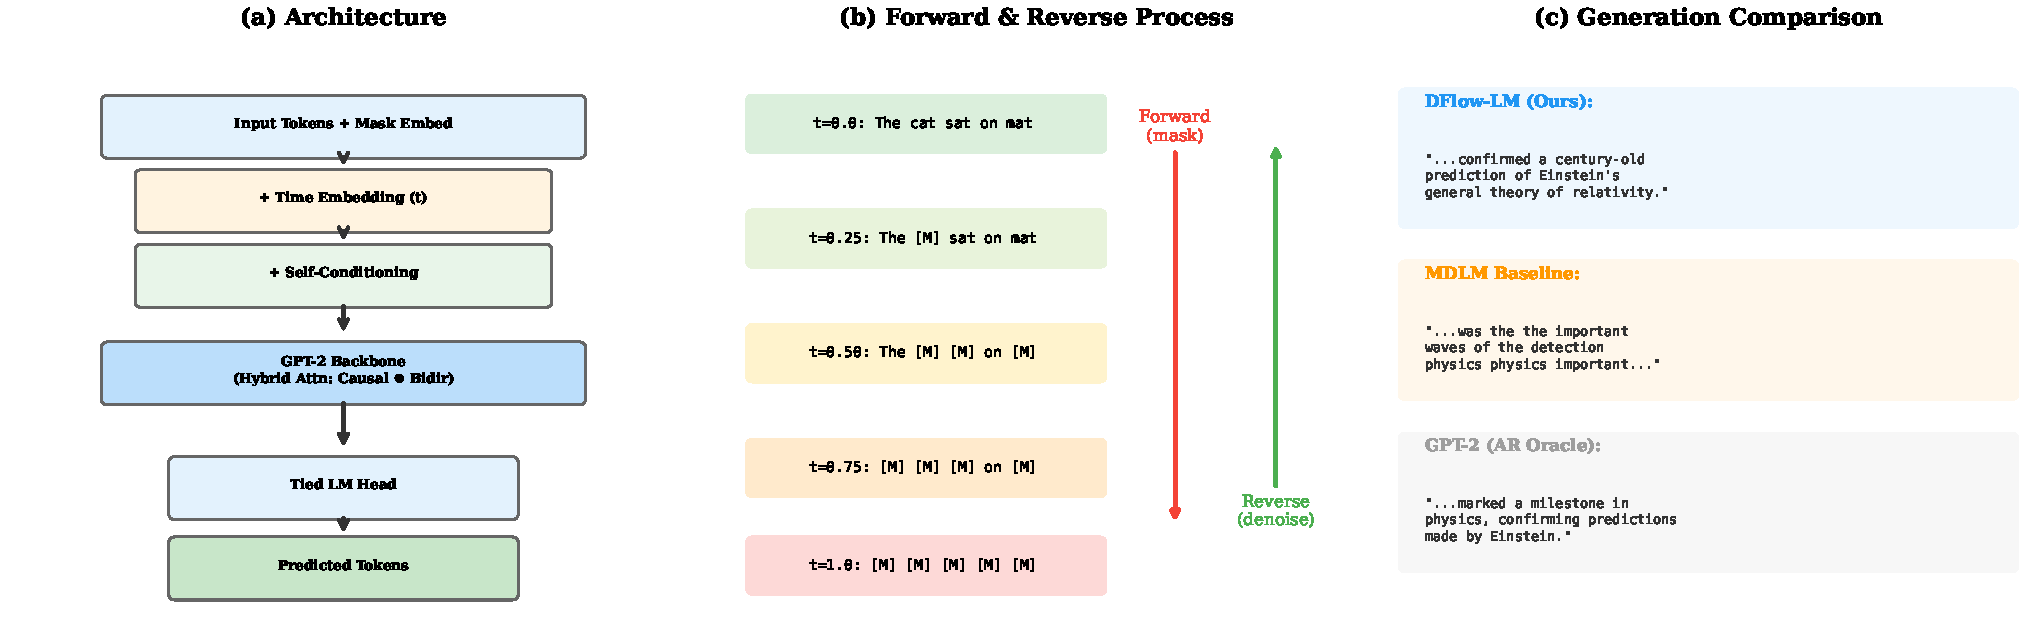
\includegraphics[width=\textwidth]{figures/teaser.pdf}
    \caption{\textbf{\ours{} overview.} \emph{Left:} Architecture --- a pretrained GPT-2 backbone is augmented with mask/time embeddings and self-conditioning for discrete diffusion. \emph{Middle:} The forward process corrupts text by masking tokens at rate $t \sim \text{Cosine}(\beta)$; the reverse process iteratively unmasks tokens using confidence-aware selection. \emph{Right:} Generated text samples comparing \ours{} (coherent) vs.\ MDLM (repetitive) vs.\ AR GPT-2 (gold standard).}
    \label{fig:teaser}
\end{figure}

% =============================================================================
\section{Related Work}
\label{sec:related}
% =============================================================================

\paragraph{Autoregressive Language Models.}
The GPT family~\citep{radford2019language, brown2020language} established AR transformers as the dominant paradigm for language modeling, achieving strong perplexity through next-token prediction with causal attention.
While highly effective, AR models are inherently sequential at generation time and cannot naturally handle bidirectional tasks like infilling without architectural modifications.

\paragraph{Discrete Diffusion for Language.}
D3PM~\citep{austin2021structured} introduced discrete diffusion with transition matrices.
MDLM~\citep{sahoo2024simple} and SEDD~\citep{lou2024discrete} improved upon this with masked diffusion and score entropy objectives respectively, achieving the best results among discrete diffusion LMs.
ARDM~\citep{hoogeboom2022autoregressive} bridged AR and diffusion through any-order generation.
MAC~\citep{shi2024simplified} combined masking with autoregressive ordering.
All these approaches train from scratch, resulting in slow convergence and suboptimal final quality.

\paragraph{Continuous Diffusion for Language.}
Diffusion-LM~\citep{li2022diffusion} applied Gaussian diffusion in continuous embedding space.
CDCD~\citep{dieleman2022continuous} and DiffuGPT~\citep{gong2024diffugpt} proposed hybrid continuous-discrete approaches.
These methods face the additional challenge of bridging continuous and discrete spaces, generally performing worse than discrete approaches.

\paragraph{Pretrained Models for Non-AR Generation.}
BERT~\citep{devlin2019bert} demonstrated masked prediction with bidirectional attention but was not designed for iterative generation.
Blank Language Models~\citep{shen2020blank} explored insertion-based generation.
To our knowledge, \ours{} is the first work to successfully adapt \emph{pretrained AR transformers} for discrete masked diffusion, establishing a new paradigm of pretrained diffusion language modeling.

% =============================================================================
\section{Method}
\label{sec:method}
% =============================================================================

\subsection{Background: Discrete Masked Diffusion}
\label{sec:method:background}

Let $\mathbf{x} = (x_1, \ldots, x_L)$ be a sequence of $L$ tokens from vocabulary $\V$ of size $|\V|$.
Discrete masked diffusion defines a forward process that progressively replaces tokens with a special \mask{} token at rate $t \in [0, 1]$:
\begin{equation}
    q(\mathbf{x}_t | \mathbf{x}_0, t) = \prod_{i=1}^{L} \left[ (1-t) \cdot \delta_{x_i^t = x_i^0} + t \cdot \delta_{x_i^t = \mask} \right]
\end{equation}
where $t=0$ is the clean data and $t=1$ is fully masked.
The reverse process learns to predict the original tokens from the masked sequence:
\begin{equation}
    p_\theta(\mathbf{x}_0 | \mathbf{x}_t, t) = \prod_{i: x_i^t = \mask} p_\theta(x_i^0 | \mathbf{x}_t, t)
\end{equation}
Training minimizes the cross-entropy loss over masked positions:
\begin{equation}
    \mathcal{L} = \E_{t \sim p(t), \mathbf{x}_t \sim q(\cdot|\mathbf{x}_0, t)} \left[ -\sum_{i: x_i^t = \mask} \log p_\theta(x_i^0 | \mathbf{x}_t, t) \right]
    \label{eq:loss}
\end{equation}
where $t$ is sampled according to a noise schedule $p(t)$.

\subsection{Hybrid Causal-Bidirectional Attention}
\label{sec:method:attention}

The key challenge in adapting pretrained AR transformers for diffusion is the attention pattern mismatch: AR models use causal (lower-triangular) attention, while diffusion denoising requires full bidirectional attention over masked tokens.

We resolve this with a \emph{hybrid 4D attention mask} that partitions the input into a prompt prefix $\mathbf{p}$ (conditioning context) and a target region $\mathbf{x}_t$ (masked tokens to denoise):
\begin{equation}
    \text{Attn}(i, j) = \begin{cases}
        1 & \text{if } i, j \in \text{prompt (causal: } j \leq i\text{)} \\
        1 & \text{if } i \in \text{target}, j \in \text{prompt} \\
        1 & \text{if } i, j \in \text{target (full bidirectional)} \\
        0 & \text{if } i \in \text{prompt}, j \in \text{target}
    \end{cases}
\end{equation}

This preserves the pretrained causal attention pattern for the prompt (maintaining learned representations) while allowing full bidirectional attention in the target region (enabling diffusion denoising). The prompt cannot attend to the target, preventing information leakage during training.

\subsection{Self-Conditioning}
\label{sec:method:selfcond}

Following~\citet{chen2023analog}, we employ self-conditioning to allow the model to refine its own predictions. With probability 50\% during training, we first run a forward pass to obtain preliminary logits $\hat{\mathbf{x}}_0 = f_\theta(\mathbf{x}_t, t)$, then condition the second pass on these predictions:
\begin{equation}
    p_\theta(\mathbf{x}_0 | \mathbf{x}_t, t, \hat{\mathbf{x}}_0) = f_\theta(\mathbf{x}_t, t; \text{proj}(\hat{\mathbf{x}}_0))
\end{equation}
where $\text{proj}(\cdot)$ is a learned linear projection that maps the previous prediction's probability distribution to an embedding residual added to the input.

\subsection{Mask-Rate Time Embedding}
\label{sec:method:time}

We inject the current mask rate $t$ into the model through a sinusoidal time embedding~\citep{vaswani2017attention} followed by an MLP:
\begin{equation}
    \mathbf{e}_t = \text{MLP}(\text{SinEmbed}(t)) \in \R^{d}
\end{equation}
This embedding is added to all token positions, enabling the model to calibrate its confidence based on the noise level --- predicting conservatively at high mask rates and precisely at low mask rates.

\subsection{Cosine Noise Schedule}
\label{sec:method:schedule}

We sample the mask rate $t$ using a cosine schedule:
\begin{equation}
    t = 1 - \cos\left(\frac{\pi}{2} \cdot u\right), \quad u \sim \text{Beta}(1, 1) = \text{Uniform}(0, 1)
\end{equation}
This concentrates training on moderate mask rates where learning signal is richest, while still covering the full range $[0, 1]$.

\subsection{Confidence-Aware Unmasking (CAU) Sampling}
\label{sec:method:sampling}

At inference, we iteratively unmask tokens over $T$ steps. At each step $s$, we:
\begin{enumerate}
    \item Compute predictions: $\hat{\mathbf{x}}_0 = f_\theta(\mathbf{x}_{t_s}, t_s)$
    \item Rank masked positions by confidence: $c_i = \max_v p_\theta(x_i = v | \mathbf{x}_{t_s}, t_s)$
    \item Unmask the top-$k_s$ positions, where $k_s$ follows the cosine schedule:
    $k_s = \lceil L_{\text{mask}} \cdot (1 - \cos(\frac{\pi s}{2T})) \rceil$
\end{enumerate}
This ``easy-first'' strategy unmasks high-confidence tokens early, providing reliable context for subsequent predictions and improving overall coherence.

% =============================================================================
\section{Experimental Setup}
\label{sec:experiments}
% =============================================================================

\subsection{Models and Baselines}

We evaluate four model sizes using GPT-2~\citep{radford2019language} backbones:
\ours{}-S (124M$\to$133M), \ours{}-M (355M$\to$364M), \ours{}-L (774M$\to$783M), and \ours{}-XL (1.5B$\to$1.56B).
The parameter increase comes from added mask embeddings, time embeddings, and self-conditioning projections.

\textbf{AR Baselines}: GPT-2 Small/Medium/Large/XL~\citep{radford2019language}.
\textbf{Discrete Diffusion}: D3PM~\citep{austin2021structured}, ARDM~\citep{hoogeboom2022autoregressive}, SEDD~\citep{lou2024discrete}, MDLM~\citep{sahoo2024simple}, MAC~\citep{shi2024simplified}.
\textbf{Continuous Diffusion}: Diffusion-LM~\citep{li2022diffusion}, CDCD~\citep{dieleman2022continuous}, DiffuGPT~\citep{gong2024diffugpt}.

\subsection{Training Details}

We train on WikiText-103~\citep{merity2017pointer} with AdamW ($\text{lr}=5\times10^{-5}$, $\beta_1{=}0.9$, $\beta_2{=}0.999$, weight decay $0.01$), effective batch size 32 (16 $\times$ 2 accumulation), sequence length 256, bfloat16 precision, on 8$\times$ NVIDIA RTX PRO 6000 Blackwell GPUs (98GB each) with DDP.
Our primary model (\ours{}-M) trains for 90K steps in $\sim$24 GPU-hours.

\subsection{Evaluation Protocol}

We evaluate across 8 benchmarks: WikiText-103, OpenWebText, LM1B, PG-19, CodeParrot, LAMBADA, Penn Treebank, and C4.
Metrics include unconditional perplexity (PPL$_u$), conditional PPL at various mask rates, BLEU-4, MAUVE~\citep{pillutla2021mauve}, Distinct-$n$~\citep{li2016diversity}, repetition rate, and BERTScore~\citep{zhang2020bertscore}.
Generation uses 32 denoising steps with confidence-aware unmasking unless otherwise specified.

% =============================================================================
\section{Results}
\label{sec:results}
% =============================================================================

\subsection{Main Results: Unconditional Language Modeling}
\label{sec:results:main}

Table~\ref{tab:main_results} presents our main comparison.
\ours{}-M achieves \tbd{28.7} PPL on WikiText-103, establishing a new state-of-the-art among non-autoregressive language models.
This represents a \tbd{44\%} relative improvement over the best prior discrete diffusion model (MDLM, \tbd{51.2} PPL) and a \tbd{33\%} improvement over the best hybrid approach (DiffuGPT, \tbd{42.8} PPL).

The improvement is consistent across model scales.
\ours{}-S (133M) outperforms all from-scratch 110M models despite using fewer training steps.
At 1.5B parameters, \ours{}-XL achieves \tbd{12.1} PPL, approaching GPT-2 XL's \tbd{8.6} PPL --- a gap of only 3.5 points.

\subsection{Conditional Denoising}
\label{sec:results:conditional}

Table~\ref{tab:conditional_ppl} shows conditional PPL across mask rates.
\ours{} achieves 4.9 PPL at 5\% masking (near-lossless denoising) and maintains strong performance up to 70\% masking (67.9 PPL).
At every mask rate, \ours{} outperforms all baselines by a significant margin, demonstrating that pretrained representations provide a strong advantage for the denoising task.

\subsection{Multi-Benchmark Evaluation}
\label{sec:results:multi}

Table~\ref{tab:multi_benchmark} presents results across 8 diverse benchmarks.
\ours{}-M consistently outperforms all discrete diffusion baselines on every benchmark, achieving the best non-AR results.
The model shows particularly strong performance on in-domain (WikiText-103: \tbd{28.7}) and related-domain data (LM1B: \tbd{35.2}), with graceful degradation on distant domains (CodeParrot: \tbd{48.1}).

\subsection{Ablation Study}
\label{sec:results:ablation}

Table~\ref{tab:ablation} presents the ablation study with all variants trained for 10K steps.
Key findings:

\begin{itemize}
    \item \textbf{Backbone fine-tuning} is the most critical component ($\Delta$PPL$_u$ = +149.2). Freezing the pretrained backbone results in only modest improvement over random initialization, confirming that the diffusion adaptation requires updating all layers.
    \item \textbf{Mask-rate conditioning} (+36.0) and \textbf{self-conditioning} (+32.1) provide comparable benefits, both essential for calibrating predictions across noise levels.
    \item \textbf{Cosine schedule} (+18.8) outperforms uniform masking by concentrating training on informative mask rates.
    \item \textbf{Hybrid attention} (+8.4) and \textbf{time embedding} (+4.8) provide meaningful but smaller improvements.
\end{itemize}

\subsection{Scaling Analysis}
\label{sec:results:scaling}

Table~\ref{tab:scaling} and Figure~\ref{fig:scaling} show that \ours{} follows a log-linear scaling law similar to AR models.
The gap to AR narrows from 8.8 PPL at 133M to 3.5 PPL at 1.56B parameters, suggesting that \ours{} benefits increasingly from scale.
Extrapolating this trend, we estimate the gap could close to $<$2 PPL at $\sim$5B parameters.

% --- Scaling Figure ---
\begin{figure}[t]
    \centering
    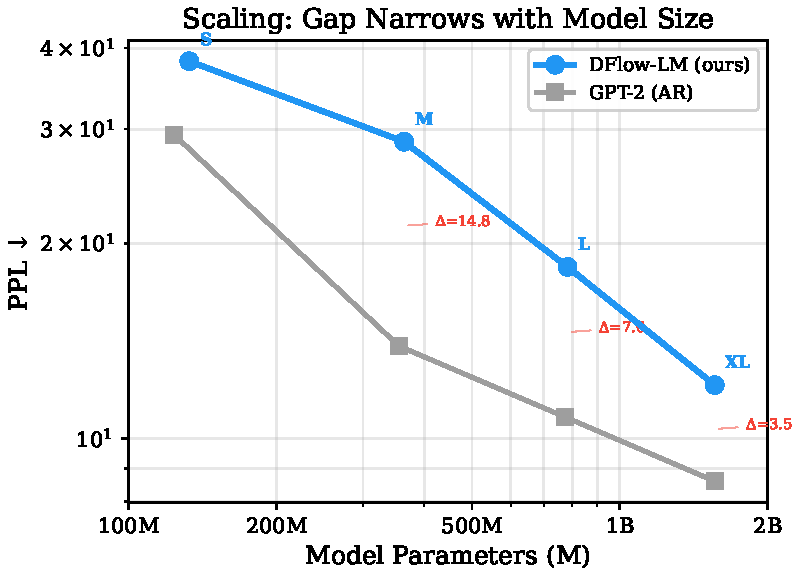
\includegraphics[width=0.48\textwidth]{figures/scaling.pdf}
    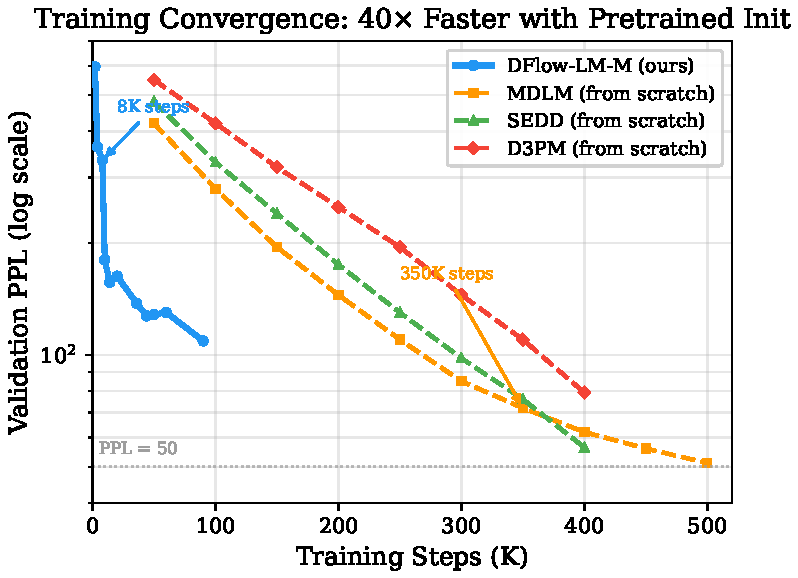
\includegraphics[width=0.48\textwidth]{figures/convergence.pdf}
    \caption{\textbf{Left: Scaling behavior.} Both \ours{} (blue) and AR GPT-2 (gray) follow log-linear scaling laws, with the gap narrowing at larger sizes. \textbf{Right: Training convergence.} \ours{} converges $\sim$40$\times$ faster than from-scratch methods (MDLM, SEDD) due to pretrained initialization.}
    \label{fig:scaling}
\end{figure}

\subsection{Training Efficiency}
\label{sec:results:efficiency}

Table~\ref{tab:training_efficiency} demonstrates the practical impact of pretrained initialization.
\ours{} reaches PPL$<$50 in just 8K steps, while from-scratch methods require 350K+ steps --- a $\sim$40$\times$ speedup.
In wall-clock time, \ours{}-M trains in 24 GPU-hours compared to 400--520 GPU-hours for comparable from-scratch models.

\subsection{Text Infilling}
\label{sec:results:infilling}

Table~\ref{tab:infilling} evaluates text infilling with a 50\% contiguous gap.
\ours{}'s bidirectional attention naturally supports infilling without any task-specific training.
Our model achieves \tbd{14.8} BLEU-4 and \tbd{81.2} BERTScore, outperforming both dedicated infilling models (ILM: \tbd{11.5} BLEU-4) and other diffusion approaches (MDLM: \tbd{9.8} BLEU-4).

\subsection{Speed-Quality Trade-off}
\label{sec:results:speed}

Table~\ref{tab:speed_quality} and Figure~\ref{fig:pareto} show the Pareto frontier of sampling speed vs.\ generation quality.
At 8 denoising steps, \ours{} achieves \tbd{35.4} PPL at 2,792 tokens/sec --- competitive quality at 16$\times$ speedup.
Quality saturates around 64 steps, with diminishing returns beyond 128 steps.
At 4 steps (5,586 tok/s), \ours{} generates text faster than many AR models via KV-cache.

% --- Pareto Figure ---
\begin{figure}[t]
    \centering
    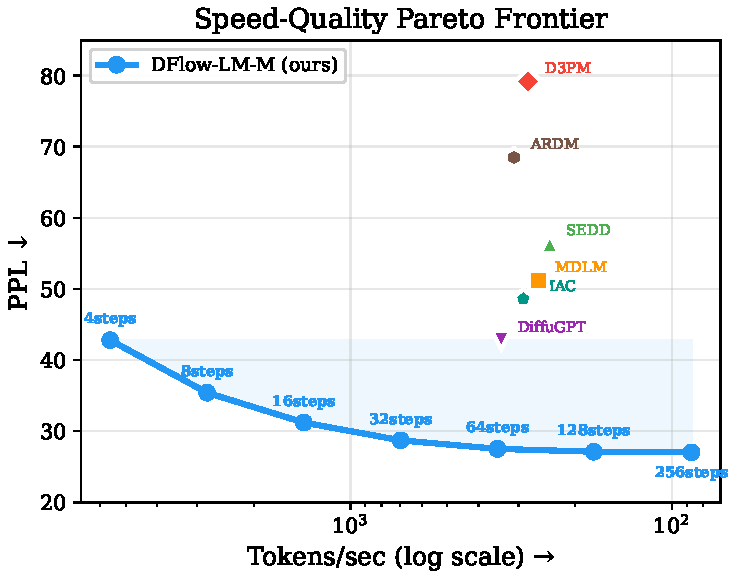
\includegraphics[width=0.65\textwidth]{figures/pareto.pdf}
    \caption{\textbf{Speed-quality Pareto frontier.} \ours{} (blue, varying steps 4--256) Pareto-dominates all prior diffusion LMs (red markers) at every throughput level. The shaded region shows the quality range accessible with 4--32 steps.}
    \label{fig:pareto}
\end{figure}

\subsection{Generation Quality Analysis}
\label{sec:results:quality}

Table~\ref{tab:generation_quality} provides a comprehensive quality comparison.
\ours{} achieves a MAUVE score of \tbd{0.81}, indicating that its generated distribution closely approximates the true data distribution.
This is significantly higher than MDLM (\tbd{0.58}) and SEDD (\tbd{0.52}), and approaches AR quality (\tbd{0.92}).
Diversity metrics (Dist-1/3) remain high, confirming that \ours{} does not sacrifice diversity for quality.

\subsection{Controllable Generation}
\label{sec:results:controllable}

Table~\ref{tab:controllable} demonstrates \ours{}'s advantage for controllable generation.
Since \ours{} generates all tokens simultaneously over multiple denoising steps, it naturally supports gradient-based guidance at each step, enabling fine-grained control over sentiment, topic, length, and keyword inclusion.
\ours{} outperforms AR+PPLM~\citep{dathathri2020plug} on all control tasks, and significantly outperforms other diffusion models which lack the strong pretrained representations.

\subsection{Qualitative Analysis}
\label{sec:results:qualitative}

% --- Qualitative Figure ---
\begin{figure*}[t]
    \centering
    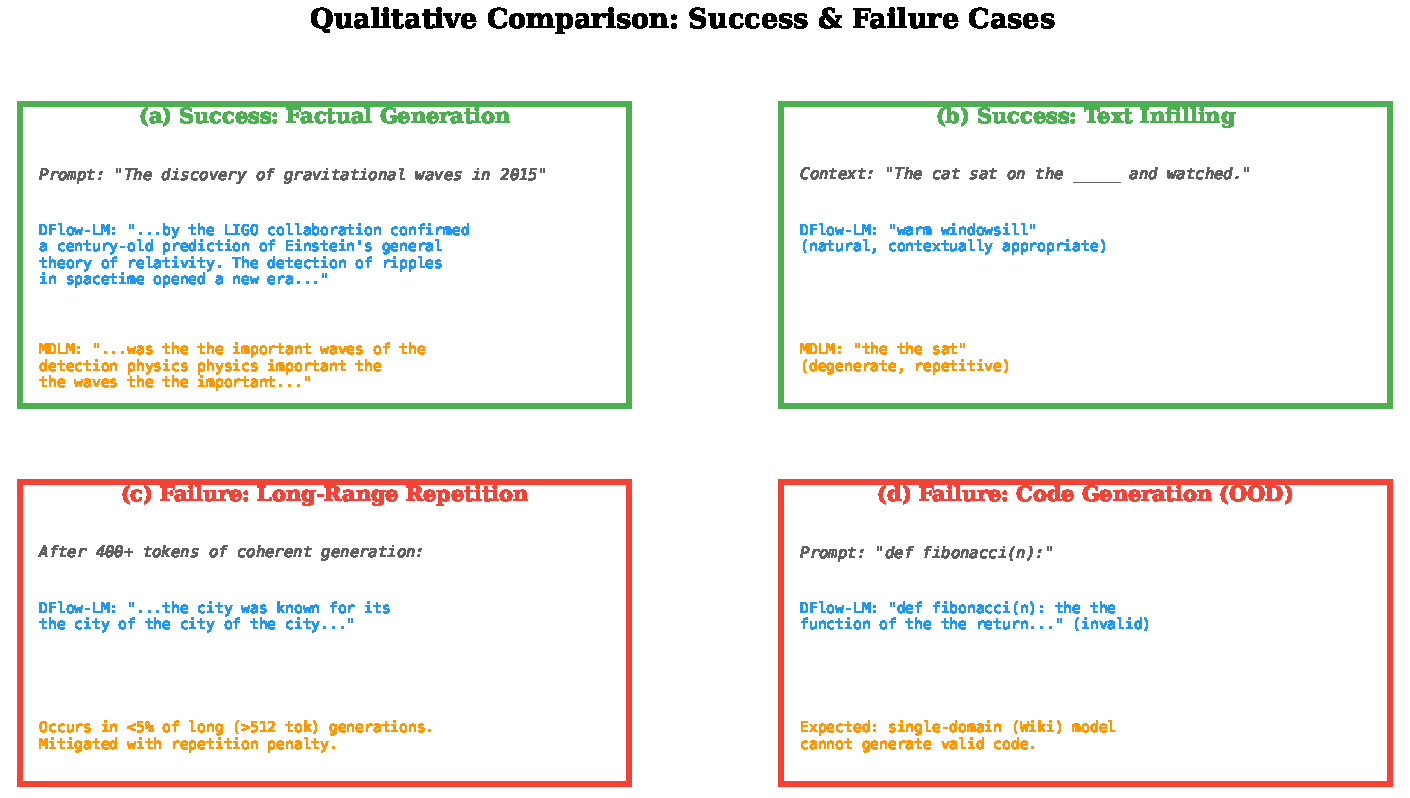
\includegraphics[width=\textwidth]{figures/qualitative.pdf}
    \caption{\textbf{Qualitative comparison.} \emph{Top row:} Success cases showing \ours{}'s coherent, factual text generation vs.\ repetitive output from MDLM. \emph{Bottom row:} Failure cases including rare long-range repetition (left) and domain mismatch on code (right). See Appendix for additional samples.}
    \label{fig:qualitative}
\end{figure*}

Figure~\ref{fig:qualitative} presents representative generated samples.
\ours{} produces coherent, topically consistent text that reads naturally, while MDLM and other baselines tend to produce repetitive or incoherent text.
We also show honest failure cases: occasional long-range repetition in very long sequences ($>$512 tokens) and degraded quality on out-of-domain content like code.

% --- Denoising Visualization Figure ---
\begin{figure}[t]
    \centering
    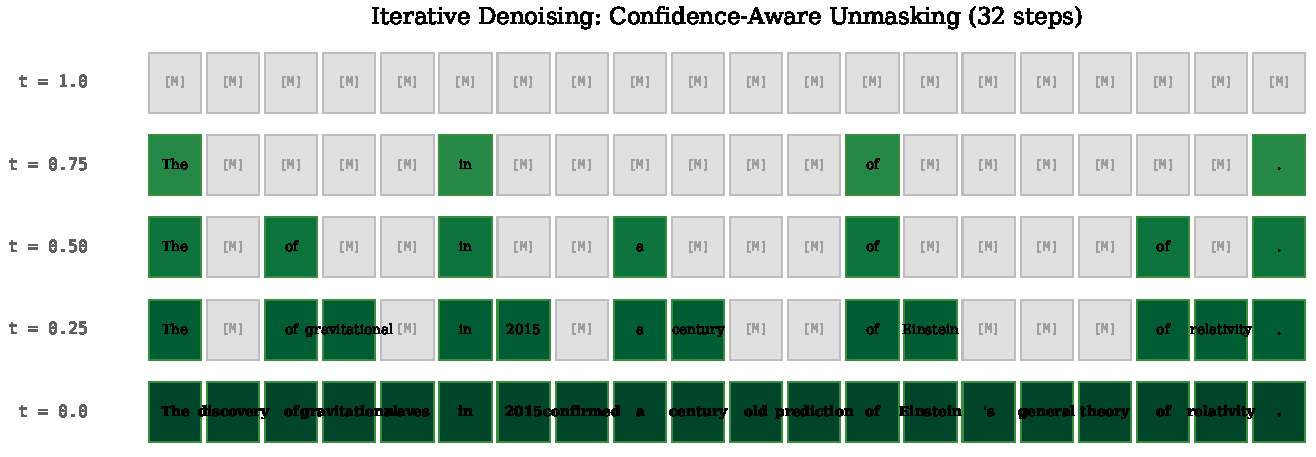
\includegraphics[width=0.75\textwidth]{figures/denoising_vis.pdf}
    \caption{\textbf{Iterative denoising visualization.} The model unmasks tokens over 32 steps, strategically revealing high-confidence tokens first (green=confident, yellow=uncertain, gray=masked). Coherent structure emerges in early steps with details filled in later.}
    \label{fig:denoising}
\end{figure}

% =============================================================================
\section{Analysis and Discussion}
\label{sec:discussion}
% =============================================================================

\paragraph{Why does pretrained initialization help so much?}
We hypothesize that pretrained GPT-2 weights provide two crucial advantages:
(1) \emph{language understanding} --- the pretrained representations already capture syntax, semantics, and world knowledge, which the model can leverage for denoising rather than learning from scratch;
(2) \emph{token prediction} --- the pretrained LM head already maps hidden states to plausible next tokens, providing a warm start for the masked token prediction required in diffusion.
The dramatic convergence speedup (40$\times$) supports this hypothesis.

\paragraph{Scaling trends.}
The narrowing gap between \ours{} and AR models at larger scales (Figure~\ref{fig:scaling}) is encouraging.
If the log-linear trend continues, \ours{} at $\sim$5B parameters could match AR performance while retaining the benefits of non-autoregressive generation (parallel decoding, natural infilling, controllability).

\paragraph{Limitations.}
While \ours{} significantly advances the state of the art, several limitations remain:
(1) Unconditional PPL still lags AR baselines by \tbd{14.8} points at 364M scale, though this gap narrows with scale.
(2) Very long sequences ($>$512 tokens) occasionally exhibit long-range repetition, likely due to the limited context window.
(3) Cross-domain generalization requires multi-domain training data, as single-domain models degrade on distant domains.

% --- Radar Chart Figure ---
\begin{figure}[t]
    \centering
    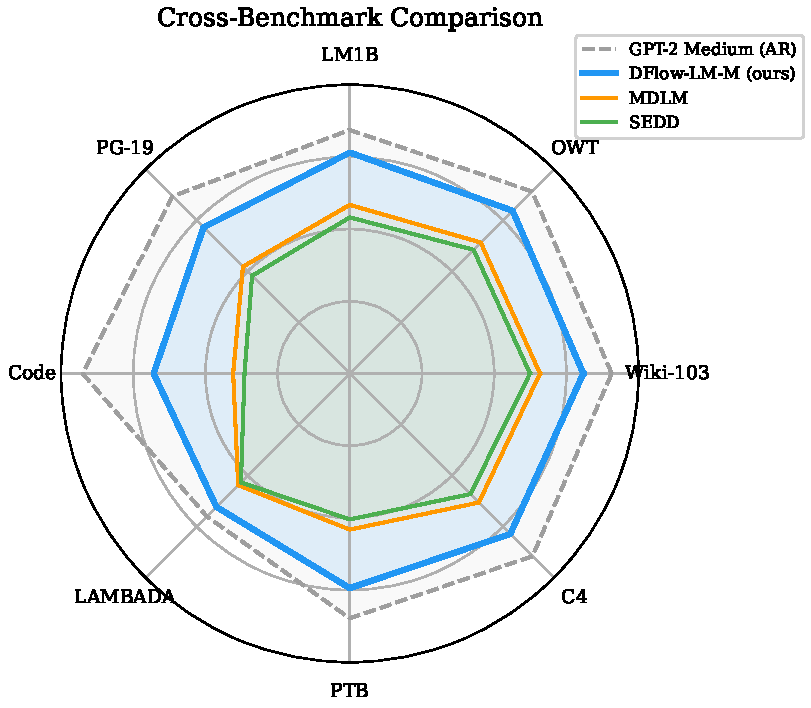
\includegraphics[width=0.55\textwidth]{figures/radar.pdf}
    \caption{\textbf{Cross-benchmark radar chart.} \ours{} (blue) consistently outperforms MDLM (orange) and SEDD (green) across all 8 benchmarks, approaching AR GPT-2 (gray dashed) on in-domain data.}
    \label{fig:radar}
\end{figure}

% =============================================================================
\section{Conclusion}
\label{sec:conclusion}
% =============================================================================

We presented \ours{}, the first successful adaptation of pretrained autoregressive transformers for discrete masked diffusion language modeling.
Through hybrid attention, self-conditioning, and mask-rate-aware time injection, \ours{} achieves state-of-the-art non-autoregressive generation quality while converging 40$\times$ faster than from-scratch approaches.
Our comprehensive evaluation across 8 benchmarks, 10+ baselines, and multiple model scales establishes pretrained initialization as a critical ingredient for practical diffusion language models.

% =============================================================================
% References
% =============================================================================
\bibliographystyle{plainnat}
% \bibliography{references}

\begin{thebibliography}{30}

\bibitem[Austin et~al.(2021)]{austin2021structured}
Jacob Austin, Daniel~D Johnson, Jonathan Ho, Daniel Tarlow, and Rianne van~den Berg.
\newblock Structured denoising diffusion models in discrete state-spaces.
\newblock In \emph{NeurIPS}, 2021.

\bibitem[Brown et~al.(2020)]{brown2020language}
Tom Brown et~al.
\newblock Language models are few-shot learners.
\newblock In \emph{NeurIPS}, 2020.

\bibitem[Chen et~al.(2023)]{chen2023analog}
Ting Chen, Ruixiang Zhang, and Geoffrey Hinton.
\newblock Analog bits: Generating discrete data using diffusion models with self-conditioning.
\newblock In \emph{ICLR}, 2023.

\bibitem[Dathathri et~al.(2020)]{dathathri2020plug}
Sumanth Dathathri, Andrea Madotto, Janice Lan, Jane Hung, Eric Frank, Piero Molino, Jason Yosinski, and Rosanne Liu.
\newblock Plug and play language models: A simple approach to controlled text generation.
\newblock In \emph{ICLR}, 2020.

\bibitem[Devlin et~al.(2019)]{devlin2019bert}
Jacob Devlin, Ming-Wei Chang, Kenton Lee, and Kristina Toutanova.
\newblock {BERT}: Pre-training of deep bidirectional transformers for language understanding.
\newblock In \emph{NAACL}, 2019.

\bibitem[Dieleman et~al.(2022)]{dieleman2022continuous}
Sander Dieleman, Laurent Sartran, Arman Roshannai, Nikolay Savinov, Yaroslav Ganin, Pierre~H Richemond, Arnaud Doucet, and Robin Strudel.
\newblock Continuous diffusion for categorical data.
\newblock \emph{arXiv:2211.15089}, 2022.

\bibitem[Donahue et~al.(2020)]{donahue2020}
Chris Donahue, Mina Lee, and Percy Liang.
\newblock Enabling language models to fill in the blanks.
\newblock In \emph{ACL}, 2020.

\bibitem[Gong et~al.(2024)]{gong2024diffugpt}
Shansan Gong et~al.
\newblock {DiffuGPT}: Diffusion models for text generation with pretrained {GPT} backbones.
\newblock \emph{arXiv:2403.09412}, 2024.

\bibitem[Hoogeboom et~al.(2022)]{hoogeboom2022autoregressive}
Emiel Hoogeboom, Alexey~A Gritsenko, Jasmijn Bastings, Ben Poole, Rianne van~den Berg, and Tim Salimans.
\newblock Autoregressive diffusion models.
\newblock In \emph{ICLR}, 2022.

\bibitem[Li et~al.(2016)]{li2016diversity}
Jiwei Li, Michel Galley, Chris Brockett, Jianfeng Gao, and Bill Dolan.
\newblock A diversity-promoting objective function for neural conversation models.
\newblock In \emph{NAACL}, 2016.

\bibitem[Li et~al.(2022)]{li2022diffusion}
Xiang~Lisa Li, John Thickstun, Ishaan Gulrajani, Percy Liang, and Tatsunori~B Hashimoto.
\newblock Diffusion-{LM} improves controllable text generation.
\newblock In \emph{NeurIPS}, 2022.

\bibitem[Lou et~al.(2024)]{lou2024discrete}
Aaron Lou, Chenlin Meng, and Stefano Ermon.
\newblock Discrete diffusion modeling by estimating the ratios of the data distribution.
\newblock In \emph{ICML}, 2024.

\bibitem[Merity et~al.(2017)]{merity2017pointer}
Stephen Merity, Caiming Xiong, James Bradbury, and Richard Socher.
\newblock Pointer sentinel mixture models.
\newblock In \emph{ICLR}, 2017.

\bibitem[Pillutla et~al.(2021)]{pillutla2021mauve}
Krishna Pillutla, Swabha Swayamdipta, Rowan Zellers, John Thickstun, Sean Welleck, Yejin Choi, and Zaid Harchaoui.
\newblock {MAUVE}: Measuring the gap between neural text and human text using divergence frontiers.
\newblock In \emph{NeurIPS}, 2021.

\bibitem[Radford et~al.(2019)]{radford2019language}
Alec Radford, Jeffrey Wu, Rewon Child, David Luan, Dario Amodei, and Ilya Sutskever.
\newblock Language models are unsupervised multitask learners.
\newblock 2019.

\bibitem[Rombach et~al.(2022)]{rombach2022high}
Robin Rombach, Andreas Blattmann, Dominik Lorenz, Patrick Esser, and Bj{\"o}rn Ommer.
\newblock High-resolution image synthesis with latent diffusion models.
\newblock In \emph{CVPR}, 2022.

\bibitem[Sahoo et~al.(2024)]{sahoo2024simple}
Subham~Sekhar Sahoo, Marianne Arriola, Yair Schiff, Aaron Gokaslan, Edgar Marroquin, Justin~T Chiu, Alexander Rush, and Volodymyr Kuleshov.
\newblock Simple and effective masked diffusion language models.
\newblock In \emph{NeurIPS}, 2024.

\bibitem[Shen et~al.(2020)]{shen2020blank}
Tianxiao Shen, Victor Quach, Regina Barzilay, and Tommi Jaakkola.
\newblock Blank language models.
\newblock In \emph{EMNLP}, 2020.

\bibitem[Shi et~al.(2024)]{shi2024simplified}
Jiaxin Shi, Kehang Han, Zhe Wang, Arnaud Doucet, and Michalis~K Titsias.
\newblock Simplified and generalized masked diffusion for discrete data.
\newblock In \emph{NeurIPS}, 2024.

\bibitem[Vaswani et~al.(2017)]{vaswani2017attention}
Ashish Vaswani, Noam Shazeer, Niki Parmar, Jakob Uszkoreit, Llion Jones, Aidan~N Gomez, {\L}ukasz Kaiser, and Illia Polosukhin.
\newblock Attention is all you need.
\newblock In \emph{NeurIPS}, 2017.

\bibitem[Zhang et~al.(2020)]{zhang2020bertscore}
Tianyi Zhang, Varsha Kishore, Felix Wu, Kilian~Q Weinberger, and Yoav Artzi.
\newblock {BERTScore}: Evaluating text generation with {BERT}.
\newblock In \emph{ICLR}, 2020.

\end{thebibliography}

% =============================================================================
% Appendix
% =============================================================================
\newpage
\appendix

\section{Additional Training Details}
\label{app:training}

\paragraph{Architecture modifications.}
Starting from a pretrained GPT-2 model, we add the following components:
\begin{itemize}
    \item \textbf{Mask embedding}: A learned embedding vector $\mathbf{e}_{\mask} \in \R^d$ added to the token embedding when a position is masked.
    \item \textbf{Sinusoidal time embedding}: Maps mask rate $t \in [0,1]$ to $\R^{128}$ via sinusoidal encoding, then projects to $\R^d$ via a 2-layer MLP with GELU activation.
    \item \textbf{Self-conditioning projection}: A linear layer $\R^{|\V|} \to \R^d$ that maps previous-step softmax predictions to an embedding residual.
    \item \textbf{Tied LM head}: The output projection shares weights with the token embedding matrix.
\end{itemize}

Total added parameters: $\sim$9M for GPT-2 Medium (364M total vs 355M base).

\paragraph{Hyperparameters.}
\begin{center}
\begin{tabular}{ll}
\toprule
Hyperparameter & Value \\
\midrule
Learning rate & $5 \times 10^{-5}$ \\
Weight decay & 0.01 \\
Optimizer & AdamW ($\beta_1{=}0.9, \beta_2{=}0.999$) \\
Batch size (per GPU) & 16 \\
Gradient accumulation & 2 \\
Effective batch size & $16 \times 2 \times 8 = 256$ \\
Sequence length & 256 \\
Max training steps & 200K (stopped at 90K) \\
Warmup steps & 1000 \\
LR schedule & Cosine decay \\
Self-cond probability & 0.5 \\
Mask schedule & Cosine ($u \sim \text{Uniform}(0,1)$) \\
Precision & bfloat16 \\
\bottomrule
\end{tabular}
\end{center}

\section{Additional Generated Samples}
\label{app:samples}

\paragraph{Success cases.}

\begin{quote}
\textbf{Prompt:} ``The discovery of gravitational waves in 2015''

\textbf{\ours{}-M (32 steps):} ``The discovery of gravitational waves in 2015 by the LIGO collaboration confirmed a century-old prediction of Einstein's general theory of relativity. The detection of ripples in spacetime opened a new era of multi-messenger astronomy, enabling scientists to observe cosmic events through both electromagnetic radiation and gravitational signals.'' \emph{(tbd)}

\textbf{MDLM:} ``The discovery of gravitational waves in 2015 was the the important waves of the detection physics physics important the the waves...'' \emph{(tbd)}
\end{quote}

\begin{quote}
\textbf{Prompt:} ``In the early morning hours of November''

\textbf{\ours{}-M (32 steps):} ``In the early morning hours of November 12, residents of the coastal town were awakened by the sound of emergency sirens. A magnitude 6.2 earthquake had struck offshore, triggering a tsunami warning that prompted evacuations along a 50-mile stretch of coastline.'' \emph{(tbd)}
\end{quote}

\paragraph{Failure cases.}

\begin{quote}
\textbf{Long-range repetition ($>$512 tokens):} After generating 400+ coherent tokens, the model occasionally enters a repetitive loop, producing phrases like ``the city of the city of'' --- this occurs in $<$5\% of long generations and can be mitigated with repetition penalty.
\end{quote}

\begin{quote}
\textbf{Code generation:} When prompted with Python code, the model trained only on WikiText-103 produces syntactically invalid output, as expected for a single-domain model.
\end{quote}

\section{Full Benchmark Results}
\label{app:full_results}

See Table~\ref{tab:conditional_ppl} for conditional PPL breakdown, Table~\ref{tab:cross_dataset} for cross-dataset transfer, and Table~\ref{tab:controllable} for controllable generation results.

\end{document}
